% Author: Rasmus Pank Roulund
\documentclass{standalone}
\usepackage{tikz}
\usetikzlibrary{shapes.geometric, arrows, positioning, calc, fit, arrows, decorations.pathreplacing}

\begin{document}

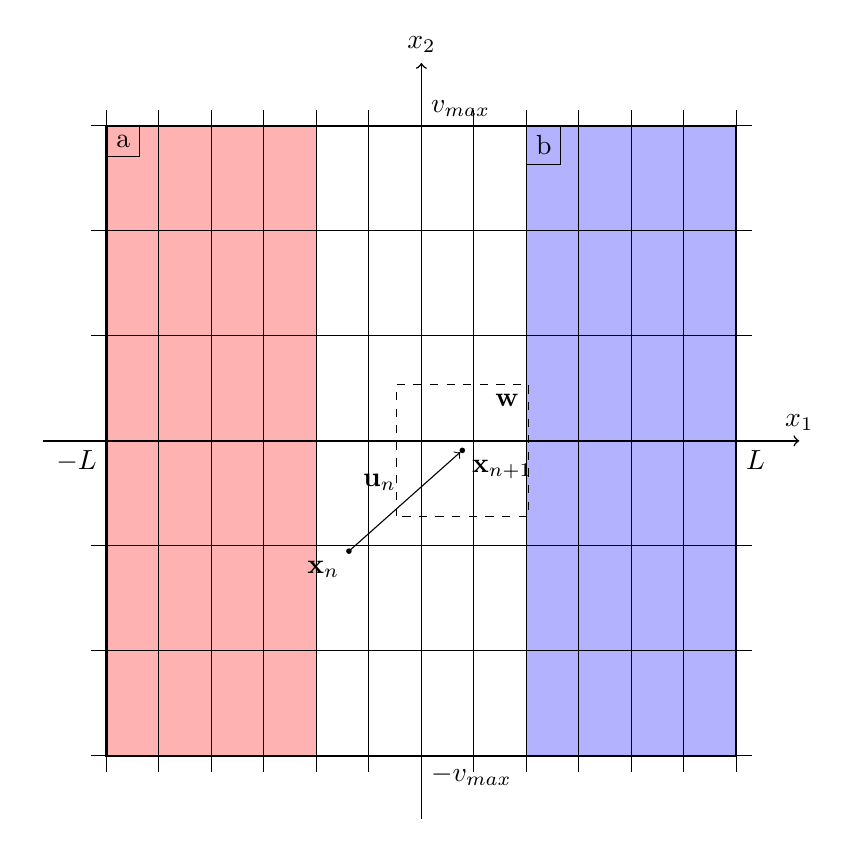
\begin{tikzpicture}[scale=4.0]


\def\outsize{1.25}
\draw[draw=none] (-\outsize,-\outsize) rectangle (\outsize,\outsize); 

\def\xd{0.25}


%\draw[step=\xd cm,gray,very thin] (-1.,-1.) grid (1.,1.);
\pgfmathsetmacro\third{1./3.}

\pgfmathsetmacro\xd{\third/2.}
\pgfmathsetmacro\yd{\third}

\def\xmax{1}
\def\xmin{-1}
\def\ymax{1}
\def\ymin{-1}

% areas
\draw[fill=blue!30!white] (\third,-1) rectangle (1.,1.);
\draw[fill=red!30!white] (-1.,-1.) rectangle (-\third,1.);

% grid
\pgfmathsetmacro\xs{\xmin+\xd}
\pgfmathsetmacro\ys{\ymin+\yd}
\pgfmathsetmacro\gridsep{0.05}
\foreach \x in {\xmin,\xs,...,\xmax} \draw (\x,\ymin-\gridsep) -- (\x,\ymax+\gridsep);
\foreach \x in {\ymin,\ys,...,\ymax} \draw (\xmin-\gridsep,\x) -- (\xmax+\gridsep,\x);

\draw[line width=0.8pt] (\xmin,\ymin) rectangle (\xmax,\xmax);

\node[draw,anchor=north west] at (\third,1) {b};
\node[draw,anchor=north west] at (-1,1) {a};

% axis
\pgfmathsetmacro\axsep{0.2}
\draw[->,line width=0.55pt] (0,\ymin-\axsep) -- (0,\ymax+\axsep) node(yaxis) [above] {$x_2$};
\draw[->,line width=0.55pt] (\xmin-\axsep,0) -- (\xmax+\axsep,0) node(xaxis) [above] {$x_1$};
        
% bounds
\node[anchor=south west] at (0,\ymax) {$v_{max}$};
\node[anchor=north west] at (0,\ymin) {$-v_{max}$};
\node[anchor=north west] at (\xmax,0) {$L$};
\node[anchor=north east] at (\xmin,0) {$-L$};

\coordinate (pt1) at (-0.23,-0.35);
\coordinate (pt2) at (0.13,-0.03);
\coordinate (w) at (0.21,0.21);

\draw[mark=*,mark size=0.2,draw=none] plot coordinates {(pt1)} -- plot coordinates {(pt2)} ;

\draw[->,shorten >=1pt]  (pt1) -- node[anchor=south east] {$\mathbf{u}_n$} (pt2) ;
\node[anchor=north east] at (pt1) {$\mathbf{x}_n$};
\node[anchor=north west] at (pt2) {$\mathbf{x}_{n+1}$};

\draw[draw,dashed] ($(pt2)-(w)$) rectangle ($(pt2)+(w)$) node[anchor=north east] {$\mathbf{w}$};

\end{tikzpicture}

\end{document}
